\chapter{Design concepts} \label{ch:design_concepts}

\section{Monolithic Architecture}

Before going into Microservices and the Microservice architecture, the Monolithic architecture approach must be explained first. The Monolithic architecture approach was till recently the preferred design option for software. In a Monolithic application all different components and functions of the business logic are combined into one indivisible program\cite{monovsmicro}. Generally these components are the user interface, business rules and data access. While individual components might be developed separately, they remain tightly coupled\cite{whatismono} and any change completed in any of them requires the whole program to be rebuild and redeployed\cite{app10175797}. More often than not development in one component requires functional changes in multiple other, adding on the development cost, complicating the build and testing process and inducing delays in deployment. A single bug in any one component can potentially halt the entire application's operation and create a nightmarish situation for on-call engineers trying to figure out the root cause and usually resulting in multiple unrelated to the issue teams joining in till root cause analysis is complete. Additionally Monolithic applications usually have large codebases, which can be cumbersome when implementing changes and difficult to manage over time\cite{whatismono}. Another major issue with Monolithic applications is scalability. Usually different components have conflicting resource requirements but because of the unified design all requirements must be handled together making scaling up the application impossible vertically, only allowing horizontal scaling through multiple copies. Scaling horizontally is very resource consuming and restricted. Finally Monolithic design allows for little to no flexibility for incorporating newer, state of the art technologies, slowly resulting in legacy applications that have to be completely redesigned and reconstructed when performance degrades. Despite the many drawbacks of Monolithic architecture, it is still favored for certain applications because of some core benefits. The most important one is performance. In most cases Monolithic applications outperform their modular counterparts\cite{whatismono}. Also initial design and implementation are easier since individual components are usually clearly defined at later stages. Additionally a single codebase and unified build and deployment process simplifies configuration management, testing and monitoring\cite{whatismono}. It is clear that the Monolithic architecture approach works well for smaller applications and helps to get things up and running faster. Furthermore when development complexity and deployment time come second to performance a Monolithic application usually has the edge over a modular approach.

\begin{figure}[!h]
    \graphicspath{ {./diagrams/} }
    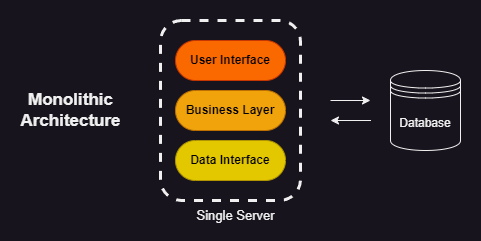
\includegraphics[scale=0.48]{monolithic_arch.png}
    \centering
    \caption{Monolithic Architecture}
    \label{fig:mono_arch}
\end{figure}

\section{Microservice Architecture}

Microservices and the Microservice Architecture are, the last few years, one of the most popular design option for software applications. In the Microservice Architecture the application is structured as a collection of independent services, called Microservices. Each Microservice corresponds to a different part of the business logic, executing a well defined unique process\cite{monovsmicro}\cite{microservicesdef}. These Microservices utilize lightweight communication mechanisms, such as API interfaces, so that they can operate in unison and achieve the same final results as a Monolithic application but without being co-depended. Microservices can be build and tested separately and be deployed and scaled independently. It's Microservice should only facilitate a single function of the application and be easily comprehensible.\cite{chandrinos_thesis}. It is not hard to understand the advantages such an architecture brings compared to it's Monolithic counterpart. Each individual Microservice can be developed separately, by different teams, without compromising or delaying the development of other parts of the application. That way, different components of the application can be improved and updated asynchronously resulting in quicker deployments of the final application and the build and deployment process is straightforward and cheaper resource wise. Also, testing is incomparably easier and faster since we don't have to build and test the whole application but only a singular Microservice. Same to testing, debugging, can be quickly and effortlessly delegated to the responsible team because it is simple to pinpoint the Microservice that failed. While all these definitely play a major factor on why the Microservice Architecture is continuously gaining in popularity, the most important advantage of it is scalability. In the era of cloud native applications where being able to scale up and down on demand is of outmost importance and where costs are usage derived, Microservice based applications significantly outclass Monolithic ones. On a Microservice application scaling is possible both vertically and horizontally. If needed the whole application can be copied just like a Monolithic one but also a single Microservice can be upscaled if demand is high. More over since Microservice applications can be readily instantiated there's no need for binding resources, opposite to Monolithic application where usually at least a couple of instances need to be always up and running to cover demand spikes resulting in exponentially increased operational costs. All these advantages, thought, cannot be achieved without drawbacks. Initial development of Microservice applications requires careful and time consuming planning and design as well as a certain level of expertise since requirements and features are not yet well defined at this stage. Also Microservice applications, more often than not, lag behind Monolithic ones in performance and therefore are not suitable for time critical operations such as load balancers. Finally, Microservice architecture is not the best option for on-prem applications where customers have to setup everything manually.\cite{whenmicroarebad}

\section{Containers}

Hand in hand with the Microservice Architecture came containers. Containers are a form of virtualization similar to virtual machines (VMs), but unlike traditional virtual machines, containers share the host system's kernel while running in isolated user spaces. This architecture makes them significantly more lightweight, efficient, and versatile compared to VMs. The primary advantage of containers lies in their efficient utilization of host hardware resources and their rapid, straightforward deployment, which is ideal for scalable environments. In comparison, Vms require a separate guest operating system, adding a large overhead both resource and time wise. Consequently, compared to VMs, containers require significantly less memory and processing power, allowing for more performance out of the same hardware infrastructure.\cite{Pahl2015} Containers are spun up from images, which are built using COntainerFiles. A ContainerFile specifies a base image and a series of steps to execute on top of it, creating what are known as layers. Each step in the build process forms a new layer, which is a critical feature for development and deployment workflows, because layers are reusable, meaning that if multiple container images share common steps, those layers need to be built only once. This reuse of layers drastically reduces build time and storage space, making containerization highly compatible with agile development processes where frequent builds and deployments are common. Container images can easily be distributed using container image registries, like Docker Hub which is the registry of the most popular container platform, Docker. Containers provide a consistent runtime environment, ensuring smooth transitions between development, staging and production environments, streamlining testing and deployment process and thus minimizing release time. Efficient use of containers, especially for application deployments, require some form of orchestration. Container orchestration is usually handled through orchestration platforms, such as Kubernetes, which automates deployment, scaling and management of containerized applications ensuring high availability, resilience and incidence recovery.\cite{dockerDev}

\section{IoT device Simulators}

There's little doubt that the Internet of Things is here to stay. IoT reshaped the way humans and machines interact with the environment and is now strongly influencing most industries. In recent years more and more everyday devices are coming equipped with all sorts of sensors and internet connectivity abilities, generating big amounts of data. Along with IoT enabled devices and sensors, there's a lot of development done on IoT applications in order to make use of all the generated data and better utilize the devices. Same as all other applications, IoT apps need to be thoroughly tested before deployment to production. One way for this to be done is to create an actual IoT network of devices, specific to the application, to generate all the data and test the application. It is not hard to notice the issues with this implementation. First of all, it is very expensive to create an actual IoT network of devices, especially when there's a need to test on large ecosystems. Furthermore, it is very common for an application early in development to be redesigned and changed often and in such case IoT ecosystem used for testing will have to be redesigned and changed as well. This adds to the development cost and introduces delays to the development process. Even if an IoT network of devices is already in place for deployment reasons, testing an application using the live network can introduce security risks. Instead of using actual data from real IoT devices, synthetic data can be generated, simulating real IoT networks. 


